% sim_results.tex -- draft of the simulation results (4 Oct 2026).
% Tables are generated by multi_drone_control/tools/thesis_sim_tables.py into Source/src/tables/,
% figures by tools/thesis_sim_figures.py (Images/*.pdf). Run ids: configs/thesis_figures.yaml.
% Cells give the mean over repeats with the number of runs in brackets.

\subsection{Carrying the payload in simulation}
\label{sec:sim_results}

The simulator is the Gazebo rig twin (Section~\ref{sec:simulation}), which reproduces the lab
set-up. It has a 0.86\,kg ring with its magnets at a radius of 0.225\,m, and 0.55\,kg UAVs on
0.55\,m rods of 0.075\,kg that pivot 4\,cm below each airframe. Thrust follows the rig's identified
affine map with battery sag, and the flight controller is a rate loop. Every flight starts
with the ring on the floor. The UAVs take off, swing their rods up to 45$^\circ$, pretension them
and lift the ring to 1.0\,m. Cases are flown twice; the tables give the number of runs in
brackets, so (1) marks a single run.

The height error is $e_z = z_L - z_L^{\mathrm{ref}}$, positive with the ring high, averaged over the
hover. The horizontal error $\|\mathbf{e}_{xy}\|$ is averaged over the first lap of a trajectory. For a
push, the displacement is measured along the push, relative to the mean over the 5\,s before it.

\subsubsection{Tracker initial condition}

Figure~\ref{fig:tracker_x0} and Table~\ref{tab:x0} compare the tracker's relaxed initial condition
($\epsilon = 0.025$) with node~0 pinned to the measurement ($\epsilon = 0$), both without integral
action.

\begin{figure}[h]
\centering
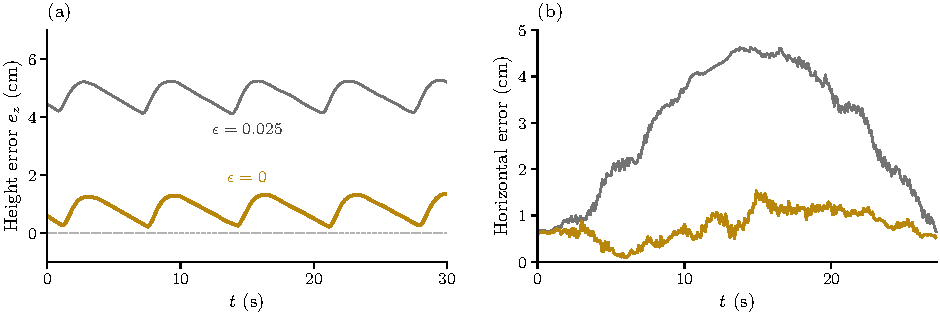
\includegraphics[width=\textwidth]{Images/tracker_x0.pdf}
\caption[Effect of the tracker's initial condition]{Effect of the tracker's initial condition without integral action: node~0 pinned to the
measured state ($\epsilon = 0$, gold) against the relaxed box ($\epsilon = 0.025$, grey). Gazebo rig
twin from a floor start, three UAVs. (a) Hover at 1.0\,m: ring height error from 10\,s after the
lift. Both settings show the same 1\,cm, 7\,s heave. (b) Circle of radius 0.5\,m at 0.125\,m/s:
horizontal ring error over the first lap including its 4\,s spin-up, sampled when the planner's
reference updates (10\,Hz). Dashed in (a): zero error. One run of each case is shown;
Table~\ref{tab:x0} gives the means.}
\label{fig:tracker_x0}
\end{figure}

\begin{table}[h]
\centering
\caption{Ring error with the relaxed and the pinned initial condition, no integral action. The
circle with $\epsilon = 0.025$ is a single run on an earlier code version; its horizontal error
reproduces on the current code (2.8\,cm, with the height integral on).}
\label{tab:x0}
% generated by tools/thesis_sim_tables.py
\begin{tabular}{llcc}
\toprule
Case & Metric & $\epsilon = 0.025$ & $\epsilon = 0$ \\
\midrule
Gazebo, hover at 1.0\,m & height error (cm) & +4.8 (2) & +0.9 (2) \\
Gazebo, circle & horizontal error, mean (cm) & 2.8 (1) & 0.8 (2) \\
 & height error (cm) & +4.8 (1) & +0.8 (2) \\
\bottomrule
\end{tabular}

\end{table}

With the box, each tracker could start its prediction from any state within 2.5\,\% of the
measured one. The solver used that freedom to treat its UAV as closer to the reference than it
was, so small errors were not corrected. Pinning node~0 brings the offset to under 1\,cm. The
remainder is attributed to
the rods' 0.075\,kg mass, which the planner does not model: they hold 52$^\circ$ instead of the
planned 45$^\circ$. This is not yet tested with node~0 pinned. With the box in place, adding the
rods' mass to the planner's model corrected the rod elevation but did not move the height.

\redo{the relaxed box against node~0 pinned on a plant that matches the controller's model (the software-in-the-loop bench, once it flies the twin), three UAVs, hover: whether the box is the whole of the height offset, and whether the rods then hold the planned 45$^\circ$ and tension.}
% --- original text, flown before the rig twin; kept to refill this place:
% With the box, each tracker could start its prediction from any state within 2.5\,\% of the
% measured one. The solver used that freedom to treat its UAV as closer to the reference than it
% was, so small errors were not corrected. In SIL, where the plant matches the model, this was the
% whole of the payload's height offset. Pinning node~0 removes it, and the rods hold the planned
% 45$^\circ$ and the planned tension. In Gazebo the offset drops to under 1\,cm. The remainder is attributed to

The box was a fraction of each \emph{absolute} coordinate, so it widened as the UAVs moved away from
the world origin. The circle's error with the box grows with the ring's distance from the origin,
which is consistent with this (Figure~\ref{fig:tracker_x0}b), although on this circle the distance and
the phase of the lap change together. Pinning node~0 also removes most of that error.

Landing is not yet resolved, with or without the box. In 21 Gazebo flights with $\epsilon = 0$, one
UAV tipped over during landing after the payload had touched down, as 2 of 32 earlier landings with the
box had. Both come from landing, not from the box, and the landing of Section~\ref{sec:sim_landing}
removes them.

\subsubsection{Disturbance rejection}

A constant force was applied to the ring for 15\,s in hover: 0.6\,N downward, about the weight of a
60\,g object, and 0.4\,N horizontally. Both were sized so that the integral stays inside its
bound, at 56\,\% and 51\,\% of it. Without an integral the ring settles 8.4\,cm and 7.6\,cm away, which gives the closed loop's
stiffness to a force on the ring: $K_z = 7.1$\,N/m and $K_{xy} = 5.3$\,N/m, the values used for
$K$ in \eqref{eq:lumped_int}. Figure~\ref{fig:disturbance} shows the model integral on the horizontal push, and
Table~\ref{tab:disturbance} gives both pushes and compares it with the target-shift form.

\begin{figure}[h]
\centering
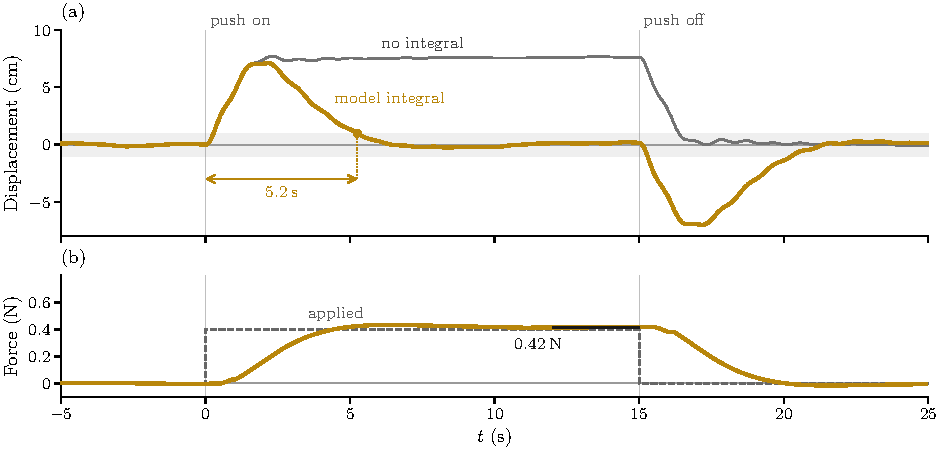
\includegraphics[width=\textwidth]{Images/disturbance.pdf}
\caption[Rejection of a constant force on the ring]{Rejection of a constant force on the ring, Gazebo rig twin, three UAVs, hover at 1.0\,m.
A 0.4\,N horizontal push acts from 0 to 15\,s. (a) Ring displacement along the push, relative to its
mean over the 5\,s before: no integral (grey) and the integral in the planner's model (gold). Band:
$\pm 1$\,cm. Arrow: time for the model integral to bring the ring back within 1\,cm for good. (b)
Change of the model integral's force $\mathbf{d}$ along the push from its value before the push
(gold), against the applied force (dashed). Black bar: its mean over the last 3\,s of the push. The
force holds still for about 0.7\,s after each step, while the ring moves faster than the integral's
5\,cm/s gate. One run of each case is shown; Table~\ref{tab:disturbance} gives the means and the
0.6\,N vertical push.}
\label{fig:disturbance}
\end{figure}

\begin{table}[h]
\centering
\caption{Disturbance rejection in the Gazebo rig twin with $\epsilon = 0$. One of the two
target-shift runs aborted on landing, after the push and its recovery; its push is included. The
change of the integral force is measured from its value before the push (0.06\,N vertically,
0.03\,N horizontally).}
\label{tab:disturbance}
% generated by tools/thesis_sim_tables.py
\small
\begin{tabular}{lccc}
\toprule
 & No integral & Target shift & Model integral \\
\midrule
\multicolumn{4}{l}{\emph{0.6\,N downward push on the ring}} \\
\quad steady displacement (cm) & 8.4 (2) & 0.3 (2) & 0.2 (2) \\
\quad peak displacement (cm) & 8.9 (2) & 6.6 (2) & 6.5 (2) \\
\quad overshoot on release (cm) & 0.4 (2) & 7.1 (2) & 7.0 (2) \\
\quad time to within 1\,cm after onset (s) & -- & 6.0 (2) & 6.1 (2) \\
\quad change of the integral force (N) & -- & -- & 0.58 (2) \\
\midrule
\multicolumn{4}{l}{\emph{0.4\,N horizontal push on the ring}} \\
\quad steady displacement (cm) & 7.6 (2) & n/a & 0.1 (2) \\
\quad peak displacement (cm) & 7.7 (2) & n/a & 7.2 (2) \\
\quad overshoot on release (cm) & 0.1 (2) & n/a & 7.0 (2) \\
\quad time to within 1\,cm after onset (s) & -- & n/a & 5.5 (2) \\
\quad change of the integral force (N) & -- & n/a & 0.42 (2) \\
\midrule
\multicolumn{4}{l}{\emph{One UAV producing more thrust than its map assumes}} \\
\quad height error (cm) & -- & 0.0 (2) & 0.0 (2) \\
\quad horizontal error (cm) & -- & 3.5 (2) & 0.0 (2) \\
\quad ring tilt (\si{\degree}) & -- & 6.4 (2) & 7.9 (2) \\
\bottomrule
\end{tabular}

\end{table}

Both forms of the integral bring the ring back to the target, and on the vertical push their
transients are the same to within a few per cent. With the conversion $K$ set to the measured
stiffness, the loop has the same gain whether the integral moves the target or enters the model. The
force the model integral learns is the force that was applied, within 3\,\% vertically and
4--5\,\% horizontally. Only the model form
acts horizontally, and it removes the horizontal push in the same way.

The integral reduces the peak only partly, by about a quarter vertically (8.9 to 6.5\,cm) and by
7\,\% horizontally (7.7 to 7.2\,cm), because it is slower than the cascade. The ring reaches most
of its uncompensated displacement within about 1\,s, while the integral's time constant is
$1/k_i = 2.5$\,s. When the push ends, the integral still holds the force it learned and drives the
ring past the target by about as much as the push displaced it at onset. This overshoot on release
is a property of integral action, not of where the integral acts. Table~\ref{tab:gain} shows the
trade-off. Doubling $k_i$ reduces the peak by 14\,\%, but the response rings and settles 55\,\% later,
the trend the damping relation of Section~\ref{sec:disturbance} predicts. This is a single run, and its
settling time is sensitive to the 1\,cm threshold against the 1\,cm heave of the hover. Keeping the
ring-speed gate only for the first 5\,s after the lift removes 7--8\,\% with no cost on this push; it has
not yet been flown on a trajectory, a hand-over or a landing.

\begin{table}[h]
\centering
\caption{Integral gain and gate on the 0.6\,N vertical push, model integral. Peak: largest
displacement during the push; overshoot and settling (to within 1\,cm): after it ends. Brackets:
number of runs.}
\label{tab:gain}
% generated by tools/thesis_sim_tables.py
\begin{tabularx}{\textwidth}{Xccc}
\toprule
Model integral & Peak (cm) & Overshoot (cm) & Settling (s) \\
\midrule
$k_i = 0.4$ & 6.5 (2) & 7.0 (2) & 4.7 (2) \\
$k_i = 0.8$ & 5.6 (1) & 6.0 (1) & 7.2 (1) \\
$k_i = 0.4$, speed gate only in the first 5\,s after the lift & 6.0 (1) & 6.4 (1) & 4.5 (1) \\
\bottomrule
\end{tabularx}

\end{table}

When one UAV produces more thrust than its map assumes, both forms hold the height. Only the model
form also removes the horizontal error, and the ring tilts 1.5$^\circ$ further. The thrust error is a
moment on the ring that neither form controls.

\redo{the two forms of the integral with the feedforward to the trackers scaled to 0.9, on a plant that matches the controller's model (the software-in-the-loop bench, once it flies the twin): the planned ring position half a second ahead against the actual one, the rod elevation, and how much of its bound the model integral uses.}
% --- original text, flown before the rig twin; kept to refill this place:
% In SIL the two forms can be compared directly, with the feedforward to the trackers scaled to 0.9.
% Both hold the target, but the reference-shift form raises the height target by 10\,cm and plans a
% climb towards it that never comes: the planned ring position half a second ahead is 4.2\,cm above
% where the ring is. The rods also settle at 48$^\circ$ rather than the planned 45$^\circ$. With the
% model integral the plan predicts what happens (0.0\,cm) and the rods hold 45$^\circ$. In SIL the model
% integral used 89\,\% of its vertical bound (0.95 of 1.07\,N) and raised its warning, because the
% conversion $K$ measured in Gazebo is lower than the SIL plant's stiffness.
% % TODO: generate the SIL plan-prediction numbers from the planner logs as the tables are.

\subsubsection{Other approaches to model error}
\label{sec:sim_methods}
% Sources: docs/overnight_2026-10-04.md (report table), registry R0841-R0955; notes 2026-10-03_*,
% 2026-10-04_* (offset_free_mpc = A, offset_free_innovation, indi_fext, kt_trim, pin_cable_rates,
% ancillary_tracker, l1_ring, xy_stiffness_b3); B4 notes 2026-10-01_load_ext_force (offline replay).
% All flown with the tracker box at 0.025 (before the x0 finding): the +4.8 cm hold is the box.

Before the initial-condition fix, several approaches from the literature were tried against the
steady errors, and each was tested in the same three-UAV rig twin. Three
cases represent the internal errors: the hover itself, and one UAV whose thrust map is wrong in
each direction (its real offset 0.03 above or below the 0.185 its tracker assumes). Two represent
external forces: a 1\,N horizontal push on the ring, and a 0.4\,m/s wind during the orbit.
Table~\ref{tab:methods} gives the results. All of them were flown with the tracker's relaxed initial
condition, so the hover without any correction sits 4.8\,cm high; the comparisons between rows still
hold.

\begin{table}[h]
\centering
\footnotesize
\setlength{\tabcolsep}{4pt}
\caption{Approaches to model error in the Gazebo rig twin (three UAVs, 1.0\,m, floor start; flown
with $\epsilon = 0.025$). Height and horizontal errors in cm, tilt in degrees; one run per cell
unless noted; a dash: not flown. $^{a}$ A UAV tipped during the landing, after the hover, and the fleet
disarmed. $^{b}$ Two runs, agreeing within 0.1.}
\label{tab:methods}
\begin{tabular}{lccccc}
\toprule
 & Hover & One UAV weaker & One UAV stronger & 1\,N push & Wind \\
 & $e_z$ & $e_z$ / $e_{xy}$ / tilt & $e_z$ / $e_{xy}$ / tilt & $e_{xy}$ & $e_{xy}$ \\
\midrule
None & +4.8 & $-$3.0 / 3.8 / 6.7 & +12.8 / 3.5 / 6.0 & 18.0 & 17.9 \\
Height integral (target) & +0.1 & 0.0 / 3.8 / 6.7 & 0.0 / 3.5 / 6.0 & 17.9 & 18.0 \\
Force balance & +3.8 & +3.9 / 1.3 / 9.0 & -- & 0.3 & 3.9 \\
Force balance + height int. & +0.1$^{b}$ & 0.0 / 1.3 / 9.0$^{b}$ & -- & 0.4$^{b}$ & 3.9$^{b}$ \\
Offset-free observer & +1.6 & +1.0 / 0.2 / 8.0 & +2.4 / 0.1 / 7.5 & 2.6$^{b}$ & 7.8$^{b}$ \\
Measured cable force & +4.2$^{a}$ & +3.8 / 3.1 / 0.8$^{a}$ & +4.5 / 0.6 / 0.3 & -- & -- \\
Measured force + height int. & 0.0$^{a}$ & 0.0 / 3.1 / 0.8 & 0.0 / 0.6 / 0.3$^{a}$ & -- & -- \\
Thrust-gain trim & +3.7 & +4.1 / 1.3 / 2.3 & -- & -- & -- \\
Rod mass in the planner & +5.0 & -- & -- & -- & -- \\
\bottomrule
\end{tabular}
\end{table}

\begin{description}
    \item[Height integral on the target.] Zeroes the height in every case and does nothing
    horizontally: the push and the wind still move the ring 18\,cm.
    \item[Force balance.] Estimates a constant force on the ring and one shared by the UAVs from
    the measured motion and the delivered thrust, and gives them to the planner's model
    \cite{muske2002disturbance}. It removes the push and most of the wind. It cannot see the internal
    height offset: by Newton's law, a force that the system exerts on itself does not appear in its
    total. It books a UAV's thrust-map error as a force on the ring, and leans the formation into
    it, which tilts the ring further. Combined with the height integral it was the best on height and
    external forces. Its transients were not small: on the push it peaked at 14.5\,cm, and on release
    it overshot by 14.8\,cm and tilted the ring 7.1$^\circ$.
    \item[Offset-free observer.] Estimates the force from the planner's own prediction error, as in
    offset-free MPC \cite{pannocchia2003disturbance}. It helped everywhere but converged slowly and left
    residuals, because a small offset shows up in the plan's cable states rather than in the payload's
    predicted motion.
    \item[Measured cable force.] Each tracker takes the cable force from its measured acceleration
    and delivered thrust, the ground-side counterpart of the IMU-based compensation of
    \cite{tudelft}. It was the only approach that levelled the ring against one UAV's wrong thrust
    map (0.3--0.8$^\circ$ against 6--7$^\circ$), because it corrects each UAV's own force. In four of
    six runs, however, a UAV tipped during the landing.
    \item[Thrust-gain trim.] A per-UAV estimate of the throttle-to-acceleration gain, from the UAV's
    own measured acceleration and its static share of the cable force. It partly corrects a wrong map.
    \item[Rod mass in the planner.] Corrected the rods' elevation (49.7 to 42.8$^\circ$ against a planned
    45$^\circ$) but not the height.
\end{description}
Further candidates were rejected before flying, because tests on logged flights showed they would
not work. These were pinning the cable rates at node~0, a thrust reference weight in the
tracker, and an $\mathcal{L}_1$ adaptive force estimate \cite{hovakimyan2010l1} at the planner's
10\,Hz rate. Raising the planner's weight on the ring's horizontal position by three and by ten times
cut the push displacement only by 23 and 38\,\% (18.5 to 14.3 and 11.4\,cm), and the higher weight
rocked the ring by 6$^\circ$. Aiming the rods at the hand-over angle instead of 45$^\circ$ made it
worse (20.7\,cm). Both were removed.

Two conclusions carried forward. First, the internal height offset was not a force at all, which is
why no force estimate could find it; it turned out to be the tracker's initial condition.
Second, a wrong thrust map on one UAV is a moment on the ring, and only a correction of that UAV's own
force removes the tilt it causes. A force on the ring, estimated or integrated, can only move the
whole formation.

\subsubsection{Trajectories}

Table~\ref{tab:traj} gives the tracking of each reference kind of Section~\ref{sec:trajectories} in
the rig twin with $\epsilon = 0$, three or four UAVs from a floor start. The integral action was off,
so the height column is the static offset that the height integral removes
(Section~\ref{sec:disturbance}). The horizontal error stays about a centimetre on average and under
3\,cm at worst for every reference, with three UAVs or four. The spin turns the ring once about its
vertical axis while it circles, and the ring follows that yaw within a few degrees.

\begin{table}[htbp]
\centering
\caption[Trajectory tracking]{Trajectory tracking in the Gazebo rig twin, $\epsilon = 0$, no integral
action, ring at 1.0\,m, floor start. Four UAVs fly the even ring except in the four-UAV hover, which
uses the detach layout. Speed: the commanded speed, which the line and the spin reach at their
peak. Horizontal error per sample, sampled where the planner's reference updates, over the motion
(the circle's first lap) or the 15\,s before LAND (hover); height error and tilt: means over the
same window; each cell is the mean over the runs.}
\label{tab:traj}
% generated by tools/thesis_sim_tables.py
\begin{tabularx}{\textwidth}{>{\raggedright\arraybackslash}Xccccccc}
\toprule
 & & Speed & \multicolumn{2}{c}{Horizontal error (cm)} & Height & Tilt & \\
\cmidrule(lr){4-5}
Reference & UAVs & (m/s) & mean & max & error (cm) & (\si{\degree}) & Runs \\
\midrule
Hover & 3 & -- & 0.7 & 0.7 & $+$0.9 & 1.2 & 2 \\
Hover, plates 1/3/5/9 & 4 & -- & 0.6 & 0.7 & $-$2.2 & 1.6 & 2 \\
Line, 1\,m shuttle & 4 & 0.25 & 0.9 & 2.7 & $-$1.7 & 1.3 & 2 \\
Circle, $r = 0.5$\,m & 3 & 0.125 & 0.8 & 1.5 & $+$0.8 & 1.2 & 6 \\
Circle, $r = 0.5$\,m & 4 & 0.125 & 0.9 & 1.9 & $-$1.7 & 1.3 & 2 \\
Figure-8, 2\,m $\times$ 1\,m & 4 & 0.25 & 0.8 & 2.4 & $-$1.7 & 1.3 & 2 \\
Spin, circle with one turn of yaw$^a$ & 4 & 0.125 & 0.5 & 1.4 & $-$1.7 & 1.2 & 2 \\
\bottomrule
\multicolumn{8}{l}{\footnotesize $^a$ Yaw error 1.3\,\si{\degree} mean, 3.5\,\si{\degree} max over the turn.}
\end{tabularx}

\end{table}

The circle and the figure-8 were also flown with the relaxed box of
Section~\ref{sec:sim_results}, $\epsilon = 0.025$ (Figure~\ref{fig:traj}). Pinning node~0 cut the
horizontal error over the motion from 3.0 to 1.0\,cm on the circle and from 2.9 to 0.8\,cm on the
figure-8, and the height error from $+3.2$ to $-1.7$\,cm. The relaxed box's error grows as the ring
moves away from the world origin and shrinks as it returns, in both shapes.

\begin{figure}[h]
\centering
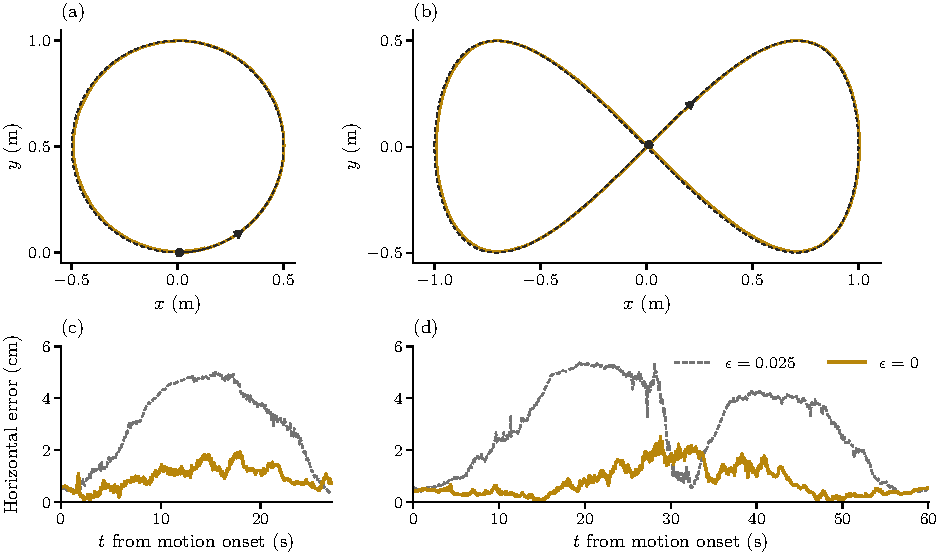
\includegraphics[width=\textwidth]{Images/trajectories.pdf}
\caption[Trajectory tracking with four UAVs]{Pinning node~0 cuts the four-UAV trajectory error by about
a factor of three. (a) Circle of radius 0.5\,m, one lap of 27\,s including a 4\,s spin-up; (b) a
2\,m\,$\times$\,1\,m figure-8 in 60\,s. Gold: ring path with $\epsilon = 0$; dark dashed: reference;
dot and arrow: start and direction. (c, d) Horizontal ring error from the onset of motion, sampled
when the planner's 10\,Hz reference updates, with $\epsilon = 0$ (gold) and the relaxed box
($\epsilon = 0.025$, dashed). Gazebo rig twin, four UAVs on the even ring, ring at 1.0\,m; one run of
each.}
\label{fig:traj}
\end{figure}

\subsubsection{Landing}
\label{sec:sim_landing}

Figure~\ref{fig:landing} compares a straight descent with the landing of
Section~\ref{sec:takeoff}, and Table~\ref{tab:land} gives every landing flown in the rig twin
with $\epsilon = 0$: three and four UAVs, hover, the pushes, the thrust-map errors, the circle and the
detach. With a straight descent, 2 of 21 landings tipped a UAV past 45$^\circ$. With the unwind alone
the outward push was gone but 2 of 18 still tipped: one survivor oscillated when the cable term
stepped off, and one departed UAV rocked on the floor. With the feedforward ramp and the ground idle
added, none of 18 tipped.

\begin{figure}[h]
\centering
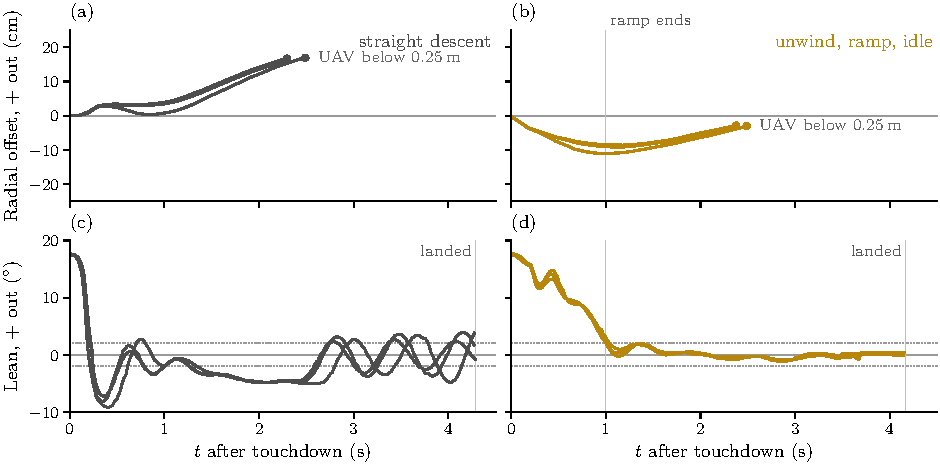
\includegraphics[width=\textwidth]{Images/landing.pdf}
\caption[Landing after touchdown]{Landing after the payload touches down, Gazebo rig twin, three
UAVs (interchangeable; one run of each). (a, c) Straight descent, with the cable feedforward cut at
touchdown. (b, d) Unwind along the rods, a 1\,s feedforward ramp and idle on the floor. (a, b) Radial
offset of each UAV from its reference about the ring centre, positive outward, drawn until the UAV
is below 0.25\,m (dot), below which its reference follows it. (c, d) Lean of each UAV's thrust axis
along its outward radial; the 17.5$^\circ$ at touchdown is the lean against the rod's pull. Dotted:
$\pm 2^\circ$. In a straight descent the rods push the UAVs outward, still growing at 17\,cm, and the
UAVs keep rocking until they land. With the unwind they trail their outward-moving reference instead
and settle within $\pm 2.6^\circ$ once the ramp ends.}
\label{fig:landing}
\end{figure}

\begin{table}[h]
\centering
\caption{Every landing in the Gazebo rig twin with $\epsilon = 0$, from load-down until the fleet is
declared landed. Tipped: a UAV past 45$^\circ$; the fleet aborts at 60$^\circ$. The ranges are over
the landings without a tip.}
\label{tab:land}
% generated by tools/thesis_sim_tables.py
\begin{tabularx}{\textwidth}{>{\raggedright\arraybackslash}Xcccc}
\toprule
Landing & Runs & Tipped (aborted) & Pushed outward (cm) & Tilt after 1.2\,s (\si{\degree}) \\
\midrule
straight descent & 21 & 2 (1) & 5.4--18.2 & 2.2--5.7 \\
unwind & 18 & 2 (2) & 0.5--4.1 & 2.4--5.0 \\
unwind, feedforward ramp, ground idle & 18 & 0 (0) & 0.5--3.0 & 1.8--4.0 \\
\bottomrule
\end{tabularx}

\end{table}

